\documentclass[tikz,border=5pt]{standalone}
\usepackage{amsmath,amssymb}
\usetikzlibrary{arrows.meta,positioning,calc,backgrounds}
\definecolor{navy}{HTML}{223D55}
\definecolor{tealbg}{HTML}{E8F3F1}
\definecolor{amberbg}{HTML}{FFF4DF}
\definecolor{amberline}{HTML}{A87B32}
\definecolor{muted}{HTML}{536674}
\definecolor{lane}{HTML}{F8FAFC}
\begin{document}
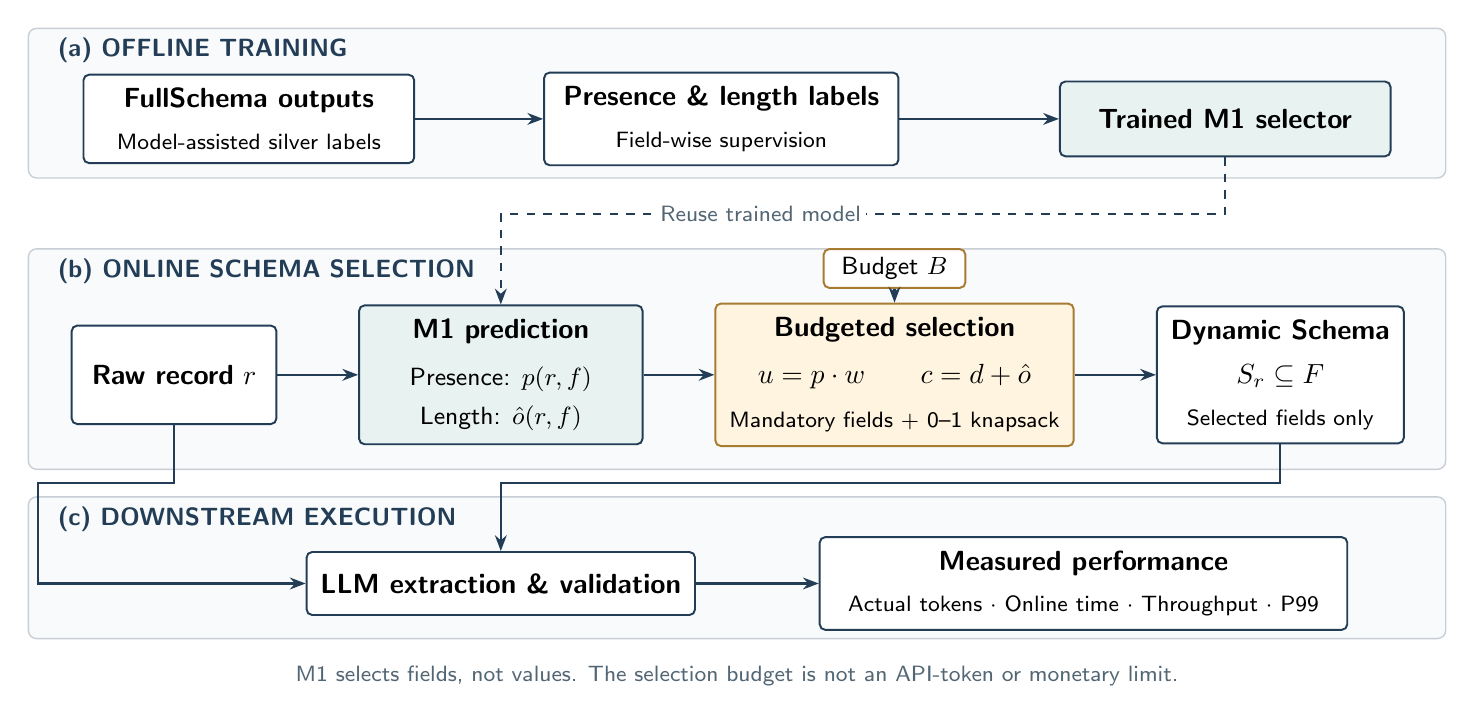
\begin{tikzpicture}[x=1cm,y=1cm,
  font=\sffamily\fontsize{10}{12}\selectfont,
  box/.style={draw=navy,line width=.7pt,rounded corners=2pt,
    fill=white,align=center,inner sep=5pt},
  flow/.style={-{Stealth[length=2mm,width=1.5mm]},draw=navy,line width=.8pt},
  dependency/.style={flow,dashed},
  heading/.style={font=\sffamily\bfseries\fontsize{9}{11}\selectfont,
    text=navy,anchor=west},
  detail/.style={font=\sffamily\fontsize{8.5}{10}\selectfont,text=muted}]
% 三层分区保持相同边界，避免背景与数据流争夺视觉注意力。
\foreach \top/\bottom in {7.5/5.6,4.7/1.9,1.55/-.25}{
  \filldraw[fill=lane,draw=navy!25,line width=.5pt,rounded corners=3pt]
    (0,\bottom) rectangle (18,\top);
}
\node[heading] at (.25,7.22) {(a) OFFLINE TRAINING};
\node[heading] at (.25,4.42) {(b) ONLINE SCHEMA SELECTION};
\node[heading] at (.25,1.27) {(c) DOWNSTREAM EXECUTION};

\node[box,minimum width=4.2cm,minimum height=.95cm] (silver) at (2.8,6.35)
  {\textbf{FullSchema outputs}\\[3pt]
   {\fontsize{8.5}{10}\selectfont Model-assisted silver labels}};
\node[box,minimum width=4.5cm,minimum height=.95cm] (labels) at (8.8,6.35)
  {\textbf{Presence \& length labels}\\[3pt]
   {\fontsize{8.5}{10}\selectfont Field-wise supervision}};
\node[box,fill=tealbg,minimum width=4.2cm,minimum height=.95cm]
  (trained) at (15.2,6.35) {\textbf{Trained M1 selector}};
\draw[flow] (silver) -- (labels);
\draw[flow] (labels) -- (trained);

\node[box,minimum width=2.6cm,minimum height=1.25cm] (raw) at (1.85,3.1)
  {\textbf{Raw record} $r$};
\node[box,fill=tealbg,minimum width=3.6cm,minimum height=1.5cm]
  (predict) at (6.0,3.1)
  {\textbf{M1 prediction}\\[5pt]
   {\fontsize{9}{11}\selectfont Presence: $p(r,f)$}\\[2pt]
   {\fontsize{9}{11}\selectfont Length: $\hat{o}(r,f)$}};
\node[box,fill=amberbg,draw=amberline,minimum width=4.55cm,
  minimum height=1.65cm] (select) at (11.0,3.1)
  {\textbf{Budgeted selection}\\[5pt]
   $u=p\cdot w\qquad c=d+\hat{o}$\\[4pt]
   {\fontsize{8.5}{10}\selectfont Mandatory fields + 0--1 knapsack}};
\node[box,minimum width=3cm,minimum height=1.5cm] (schema) at (15.9,3.1)
  {\textbf{Dynamic Schema}\\[4pt]
   $S_r\subseteq F$\\[3pt]
   {\fontsize{8.5}{10}\selectfont Selected fields only}};
\draw[flow] (raw) -- (predict);
\draw[flow] (predict) -- (select);
\draw[flow] (select) -- (schema);
% 训练模型以虚线表示依赖，不与在线记录的数据流混淆。
\draw[dependency] (trained.south) -- (15.2,5.14) -- (6,5.14) -- (predict.north);
\node[detail,fill=white,inner sep=2pt] at (9.3,5.14) {Reuse trained model};
\node[box,draw=amberline,minimum width=1.8cm,inner sep=3pt,
  font=\sffamily\fontsize{9}{11}\selectfont] (budget) at (11,4.45) {Budget $B$};
\draw[flow] (budget.south) -- (select.north);

\node[box,minimum width=4.7cm,minimum height=.8cm] (llm) at (6,.45)
  {\textbf{LLM extraction \& validation}};
\node[box,minimum width=6.7cm,minimum height=.95cm] (metrics) at (13.4,.45)
  {\textbf{Measured performance}\\[3pt]
   {\fontsize{8.5}{10}\selectfont Actual tokens $\cdot$ Online time $\cdot$ Throughput $\cdot$ P99}};
% 原始记录与所选 Schema 均输入 LLM；性能只从下游执行获得。
\draw[flow] (raw.south) -- (1.85,1.73) -- (.12,1.73)
  -- (.12,.45) -- (llm.west);
\draw[flow] (schema.south) -- (15.9,1.73) -- (6,1.73) -- (llm.north);
\draw[flow] (llm.east) -- (metrics.west);
\node[detail,anchor=north,align=center] at (9,-.48)
  {M1 selects fields, not values.
   The selection budget is not an API-token or monetary limit.};
\end{tikzpicture}
\end{document}
